\documentclass{article}
\usepackage[T1]{fontenc}

\usepackage{graphicx}
\usepackage{listings}
\begin{document}

\title{FOSS Lab Report}
\author{Gokul K\\[2\baselineskip]
Roll Number: 21\\[2\baselineskip]}
\date{19 January 2020}

\maketitle

\section{Basic Linux Commands}
\subsection{Aim}
To familiarise basic linux commands for directory and file operations
\subsection{Commands}
\subsubsection{Creating and opening a directory}
Linux terminal has a directory known as present working directory. Normally it is the home directory, but it can be changed to open any directory. Any command when destination is not specified will operate on the current working directory

\begin{enumerate}
    \item {\bf pwd}: Used to output the present working directory\newline
    \hspace{\parindent} {\em usage}: pwd
    
    \item {\bf mkdir}: Used to create directories\newline
    \hspace{\parindent} {\em usage}: mkdir directory
    
    \item {\bf cd}: Used to change the present working directory\newline
    \hspace{\parindent} {\em usage}: cd directory
    
    \begin{figure}
        \centering
        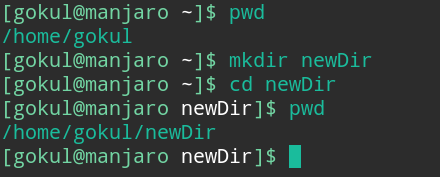
\includegraphics[width=.80\textwidth]{img/p1/ss1.png}
        \caption{Sample input/output of above commands}
    \end{figure}
\end{enumerate}

\subsubsection{Listing the contents of a directory}
\begin{enumerate}
    \item {\bf ls}: Used to list the the contents in a folder\newline
    \hspace{\parindent}{\em options} 
    \newline-a : Do not ignore items starting with .
    \newline-l : Use a long listing format with more details
    \newline-h : To display file sizes in human readable format
    \newline-f : Mark all executables with * and directories with /\newline
    \hspace{\parindent} {\em usage}: ls [options] [directory] \newline
    
\end{enumerate}
    \begin{figure}[h]
        \centering
        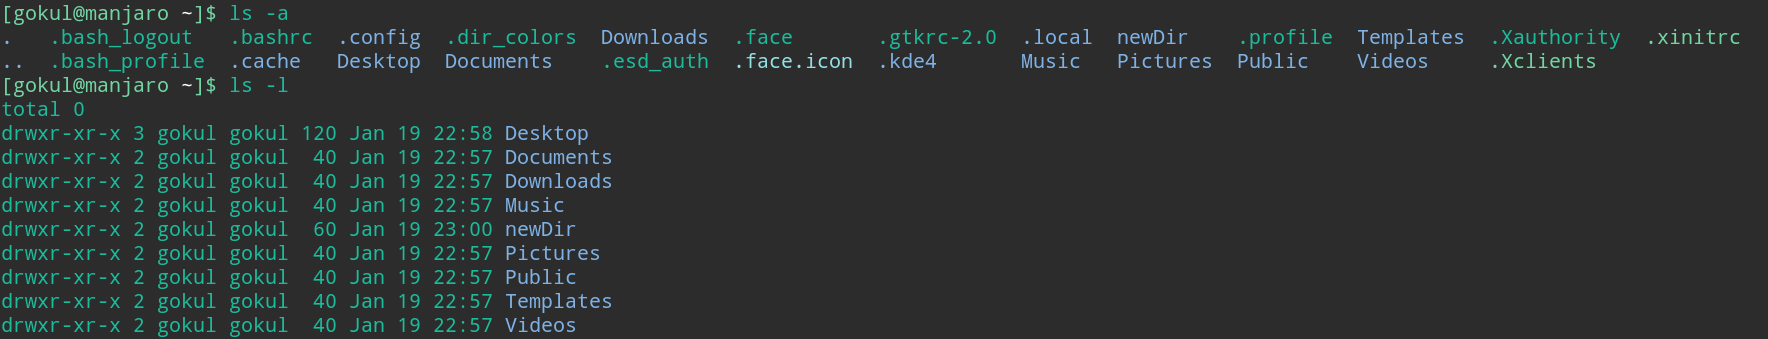
\includegraphics[width=.80\textwidth]{img/p1/ss2.png}
        \caption{Sample input/output of ls command}
    \end{figure}
    
\subsubsection{Creating and opening files}
\begin{enumerate}
    \item {\bf touch}: Changes the timestamps of a file, creates a file if it does not exists\newline
    \hspace{\parindent} {\em usage}: touch filename
    
    \item {\bf cat}: Used to output the contents of a file to the standard output\newline
    \hspace{\parindent} {\em usage}: cat filename
    
    \item {\bf more}: Used to view the contents of a text file one screen at a time.\newline
    \hspace{\parindent} {\em usage}: more filename
    
    \item {\bf less}: Used to view the contents of a text file one screen at a time. Faster than more since whole file is not loaded at once\newline
    \hspace{\parindent} {\em usage}: less filename
    \begin{figure}[h!]
        \centering
        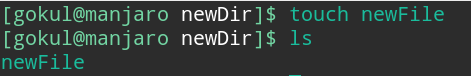
\includegraphics[height=.18\textwidth, width=.83\textwidth]{img/p1/ss3.png}
        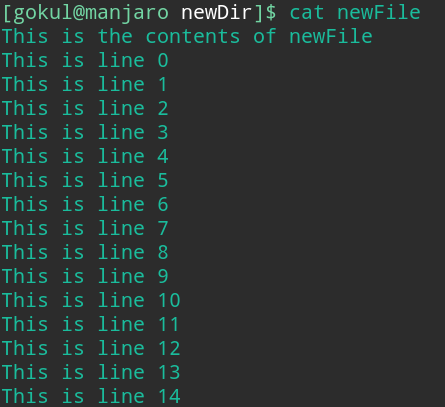
\includegraphics[height=.40\textwidth]{img/p1/ss06.png}
         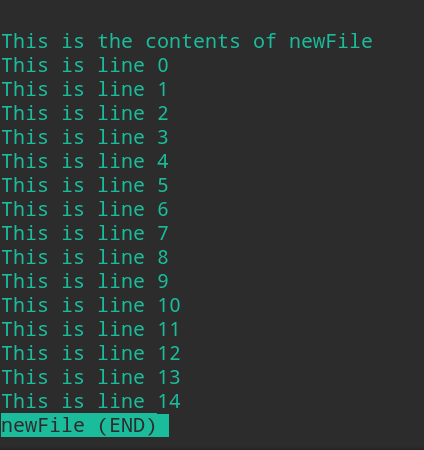
\includegraphics[height=.40\textwidth]{img/p1/ss07.png}
        \caption{Sample input/output of file commands}
    \end{figure}
\end{enumerate}

\subsubsection{Copying and deleting files and folders}
\begin{enumerate}
    \item {\bf cp}: Copies the file from source to destination. Option -r should be used to copy folders recursively. If destination is a folder, the contents are copied as children of that folder\newline
    \hspace{\parindent} {\em usage}: cp [options] source destination
    
    \item {\bf rm}: Used to remove files and folders. Use -r to remove folders recursively\newline
    \hspace{\parindent} {\em usage}: rm [options] location
    
    \begin{figure}[h!]
        \centering
        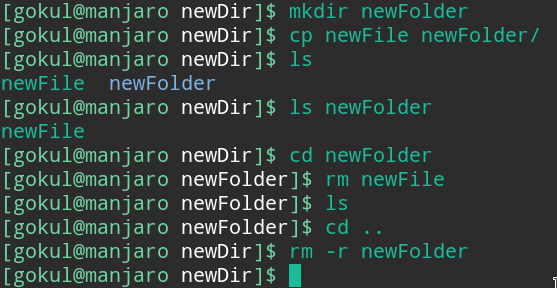
\includegraphics[width=.83\textwidth]{img/p1/ss04.png}
        \caption{Sample input/output of cp/rm commands}
    \end{figure}
\end{enumerate}

\subsubsection{Permissions}
\begin{enumerate}
    \item {\bf chmod}: Used to change the access permission of filesystem objects. Each digit in mode represent owner, group, others respectively. The mode digit can be found out by calculation decimal equivalent of rwx binary\newline
    \hspace{\parindent} {\em usage}: chmod [options] mode location
    
    \item {\bf chown}: Used to change the owner of the filesystem object\newline
    \hspace{\parindent} {\em usage}: chown [options] newowner location
    
    \item {\bf chgrp}: Used to change the file group ownership of the filesystem object\newline
    \hspace{\parindent} {\em usage}: chgrp [options] newgroup location
    
    \item {\bf su}: To temporarily become super user\newline
    \hspace{\parindent} {\em usage}: su
    
    \begin{figure}[h!]
        \centering
        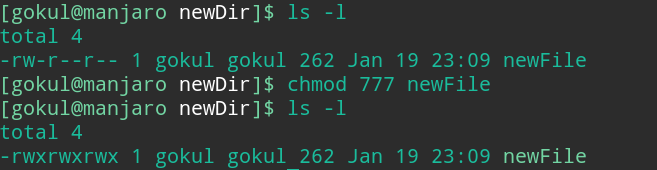
\includegraphics[width=.83\textwidth]{img/p1/ss10.png}
        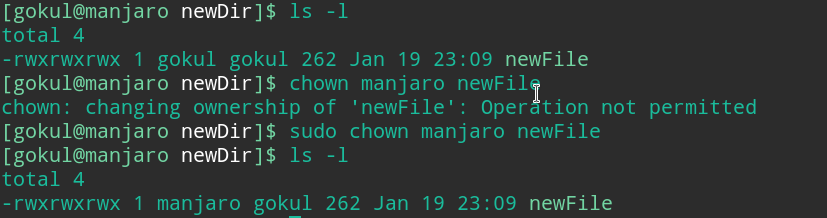
\includegraphics[width=.83\textwidth]{img/p1/ss11.png}
        \caption{Sample input/output of permission commands}
    \end{figure}
\end{enumerate}


\subsubsection{Manual pages}
\begin{enumerate}
    \item {\bf man}: Used to output the manual page of each command\newline
    \hspace{\parindent} {\em usage}: man command\newline
    
\end{enumerate}
    \begin{figure}[h]
        \centering
        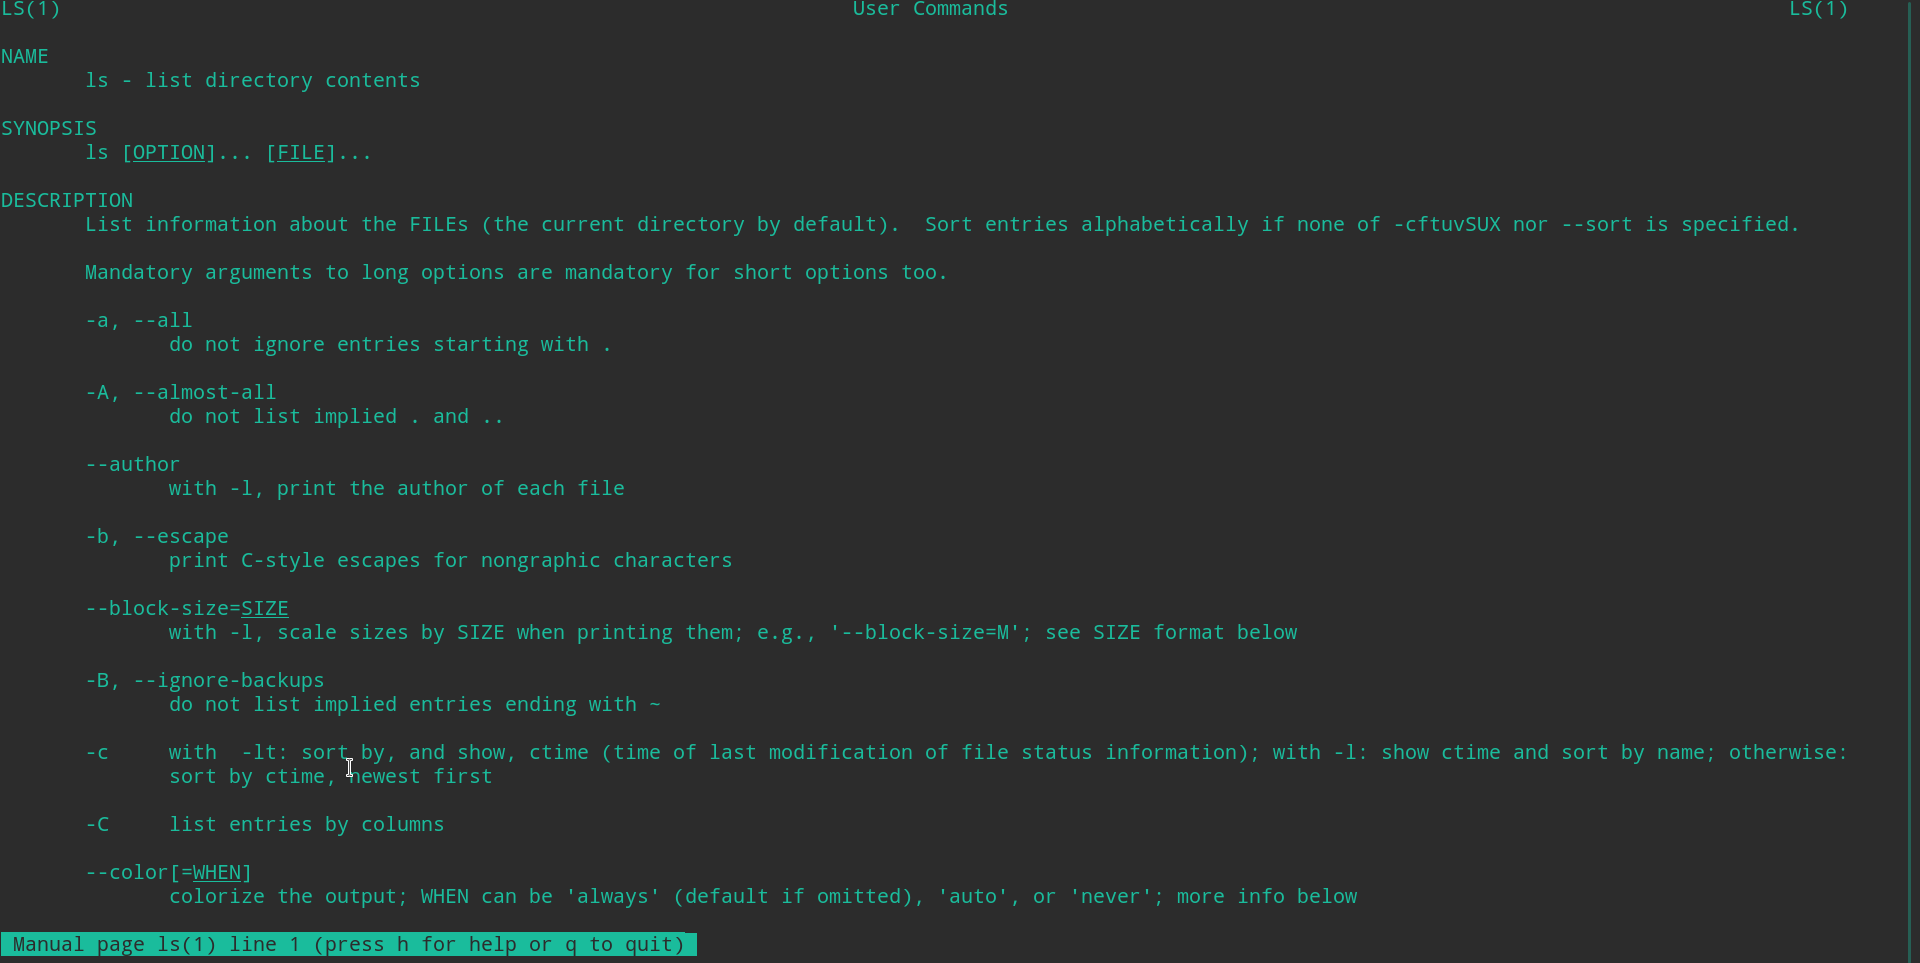
\includegraphics[width=.80\textwidth]{img/p1/ss05.png}
        \caption{Manual page of ls command}
    \end{figure}
    

\subsection{Result}
The above commands are executed and output is verified
\end{document}